\documentclass[xetex,xcolor={table,usenames,dvipsnames}]{beamer}
\usepackage{ragged2e} % Ensure ragged2e is included
\usepackage{beamerthemesplit}
\usepackage[utf8]{inputenc}
\usepackage{ccicons}
\usepackage[T1]{fontenc}
\usepackage[english,french]{babel}
\usepackage{times}
\usepackage{tabularx}
\usepackage{tabularray}
\UseTblrLibrary{booktabs, siunitx}
\usepackage{dsfont}
\usepackage{textcomp}
\usepackage{amssymb}
\usepackage{array}
\usepackage{soul}
\usepackage{amsmath}
\usepackage{graphicx}
\usepackage{bbding}
\usepackage{listings}
\definecolor{mygray}{rgb}{0.8,0.8,0.8}
\lstset{%
	basicstyle=\ttfamily,
	breaklines = true,
	backgroundcolor=\color{mygray},
}
\usepackage{realboxes}

\DeclareDocumentCommand{\clist}{v}{%
	\Colorbox{mygray}{\csname lstinline\endcsname!#1!}%
}
\usepackage[absolute,overlay]{textpos}
\usepackage[style=authoryear, maxbibnames=99, mincitenames=1, maxcitenames=2, backref=true, hyperref=true, dashed=false, firstinits=true, backend=bibtex, bibencoding=utf8, uniquename=false, uniquelist=false, natbib=true]{biblatex}
\renewcommand*{\bibfont}{\scriptsize}
\setbeamerfont{footnote}{size=\tiny}

% Remove quotation marks from titles
\DeclareFieldFormat[article,incollection,inproceedings,conference]{title}{#1} 

\usepackage{makecell}

\usepackage{capt-of}

\usepackage{xcolor}
\usepackage{shadowtext} 
% Define a custom color for lavender
\definecolor{lavender}{RGB}{230,230,250}
\definecolor{deepred}{RGB}{201,10,77}
\definecolor{deepblue}{RGB}{55,66,136}

\usepackage{hyperref}
 
 \hypersetup{
    colorlinks=true,      % Enable colored links
   linkcolor=violet,        % Color for internal links (sections, equations, etc.)
    citecolor=BlueViolet,      % Color for citations
    filecolor=magenta,    % Color for file links
    urlcolor=blue         % Color for URLs
}

\mode<presentation>
{
\usetheme{metropolis}


\setbeamercolor{header}{bg=MidnightBlue, fg=white} % Dark theme header
\setbeamercolor{progressdots}{fg=white} % Color for navigation dots

\setbeamertemplate{headline}{%
	% First row: Section Titles
	\begin{beamercolorbox}[wd=\paperwidth,ht=2.5ex,dp=1ex,center]{header}
		\textbf{\insertsectionnavigationhorizontal{\paperwidth}{}{}}
	\end{beamercolorbox}
	
	% Second row: Navigation Dots (one per frame under each section)
	\begin{beamercolorbox}[wd=\paperwidth,ht=1.5ex,dp=0ex,center]{progressdots}
		\hspace{5pt} % Adjust spacing
		\foreach \sec in \inserttotalsections { % Loop through sections
			\foreach \fr in {1,...,\insertsectionframe} { % Loop through frames in section
				\ifnum\fr=\insertframeinsection
				{\color{white}●} % Highlight current frame in section
				\else
				{\color{gray}○} % Other frames in section
				\fi
				\hspace{3pt} % Adjust spacing between dots
			}
			\hspace{10pt} % Space between sections
		}
	\end{beamercolorbox}
}

\setbeamertemplate{footline}{%
	\begin{beamercolorbox}[wd=\paperwidth,ht=2.5ex,dp=1ex,leftskip=3mm,rightskip=3mm]{footline}
		\hspace{3mm} \textbf{Ljudmila PETKOVI\'C} \hfill
		\textbf{\textsc{M2SOL034} : Reconnaissance des entités nommées (\textsc{REN})} \hfill
		\textbf{\today} \hspace{3mm}
	\end{beamercolorbox}%
}


\setbeamertemplate{headline}{%
	\begin{beamercolorbox}[wd=\paperwidth,ht=2ex,dp=1ex,center]{frametitle}
		\insertsectionnavigationhorizontal{\paperwidth}{}{}
	\end{beamercolorbox}%
}
\setbeamertemplate{footline}{%
	\begin{beamercolorbox}[wd=\paperwidth,ht=4ex,dp=1ex,leftskip=3mm,rightskip=3mm]{footline}
		\hspace{3mm} 
		\textcolor{gray}{\textbf{Ljudmila PETKOVI\'C}} \hfill
		\textcolor{gray}{\textbf{\textsc{M2SOL034} : Reconnaissance des entités nommées (\textsc{REN})}} \hfill 
		\textcolor{gray}{\textbf{\today}} \hspace{3mm}
		\textcolor{gray}{\textbf{\insertframenumber{} / \inserttotalframenumber}} \hspace{3mm} % Page number in bottom-right
	\end{beamercolorbox}%
	
	% Add the logo only if we're NOT on the title slide
	\ifnum\insertframenumber>0
	\begin{textblock*}{2.5cm}(\paperwidth-2cm,1\textheight) % Move slightly down and right
		
\includegraphics[width=1.2cm]{img/logo.png} % Adjusted logo size
	\end{textblock*}
	\fi
}









%\usecolortheme{beaver}
\usefonttheme{professionalfonts}
}







\usepackage{listings}

\lstset{ 
  language=C,                     % Set language
  basicstyle=\ttfamily\small,      % Set basic style to small monospaced font
  keywordstyle=\color{blue},       % Set keywords in blue
  commentstyle=\color{gray},       % Set comments in gray
  stringstyle=\color{red},         % Set strings in red
  numbers=left,                    % Line numbers on the left
  numberstyle=\tiny\color{gray},   % Style for line numbers
  stepnumber=1,                    % Line number step
  showstringspaces=false,          % Don't show spaces in strings
  tabsize=4,                       % Set tab size
  breaklines=true,                 % Break long lines
  captionpos=b                     % Caption position bottom
}

\usepackage[font=scriptsize,justification=centering]{caption}
\setbeamercolor{normal text}{fg=black,bg=black}
\setbeamercolor{frametitle}{fg=purple,bg=white}
\setbeamercolor{background canvas}{bg=white}
\setbeamercolor{title}{fg=purple}
\setbeamercolor{subtitle}{fg=purple}
\setbeamercolor{section in toc}{fg=purple}
\setbeamercolor{footline}{fg=purple,bg=white}
%\setbeamercolor{block title}{fg=purple,bg=white}
%\setbeamercolor{block body}{fg=white,bg=black}

\newcommand{\bolder}[1]{{\color{purple}\bfseries#1}}

% Set bullet points color to gold
\setbeamercolor{itemize item}{fg=violet}
\setbeamercolor{itemize subitem}{fg=violet}
\setbeamercolor{itemize subsubitem}{fg=violet}


\beamertemplatetransparentcovered
\beamerboxesdeclarecolorscheme{myalert}{red}{black!5!averagebackgroundcolor}
\beamerboxesdeclarecolorscheme{mybox}{blue}{black!5!averagebackgroundcolor}


%% Customize the colors for the footer
%\setbeamercolor{footline}{bg=white,fg=violet} % Set background to violet and text to white
%\setbeamercolor{footline title}{bg=white,fg=violet}
%\setbeamercolor{footline section}{bg=white,fg=violet}
%\setbeamercolor{footline page}{bg=white,fg=violet}
%
%% Customize the footer
%\setbeamertemplate{footline}{%
%  \leavevmode%
%  \hbox{%
%    \begin{beamercolorbox}[wd=.333\paperwidth,ht=2.25ex,dp=1ex,leftskip=3mm,rightskip=3mm,center]{footline title}%
%      \usebeamerfont{author in head/foot}\insertshorttitle
%    \end{beamercolorbox}%
%    \begin{beamercolorbox}[wd=.333\paperwidth,ht=2.25ex,dp=1ex,center]{footline section}%
%      \usebeamerfont{author in head/foot}\insertsection
%    \end{beamercolorbox}%
%    \begin{beamercolorbox}[wd=.333\paperwidth,ht=2.25ex,dp=1ex,right,center]{footline page}%
%      \usebeamerfont{author in head/foot}\insertframenumber{} / \inserttotalframenumber
%    \end{beamercolorbox}%
%  }%
%  \vskip0pt%
%}

\setbeamercolor{block title}{bg=violet,fg=white}
\setbeamercolor{block body}{bg=lavender,fg=black}


 \newcommand{\cf}{\textit{cf.} }
 \newcommand{\ie}{\textit{i.e.} }
 \newcommand{\ev}{espace vectoriel }
 \newcommand{\ssi}{si et seulement si }




\newcommand{\espc}[1]{\esp\left[ #1 \right]}

\newcommand{\defe}{\stackrel{\mbox{\begin{tiny}
 déf
 \end{tiny}}}{=}}
 \newcommand{\tend}[2]{\mathop{\longrightarrow}\limits_{#1\rightarrow #2}}

\newcommand{\rem}{\noindent\textbf{Remark : }}
\newcommand{\rems}{\textbf{Remarques: }}

\newcommand{\exs}{\textbf{Exemples: }}

\newcommand{\imp}[1]{\textbf{\textit{#1}}}


%\newtheorem{lem}{\textbf{Lemma}} 
%\newtheorem{theo}{\textbf{Theorem}} %[section]
%\newtheorem{prop}{\textbf{Proposition}}%[chapter]
%\newtheorem{coro}{\textbf{Corollary}}%[chapter]
%\newtheorem{hyp}{\textbf{Hypothesis}}
%\newtheorem{defi}{\textbf{Definition}}
%\newtheorem{pdefi}{\textbf{Proposition-D\'{e}finition}}

%\newenvironment{proof}[1][Proof : ]{\begin{trivlist}
%\item[\hskip \labelsep {\bfseries #1}]}{\hfill $\Box$\end{trivlist}}
%
%\newtheorem{lem}{\textbf{Lemme}} 
%\newtheorem{theo}{\textbf{Théorème}} %[section]
%\newtheorem{prop}{\textbf{Proposition}}%[chapter]
%\newtheorem{coro}{\textbf{Corollaire}}%[chapter]
%\newtheorem{hyp}{\textbf{Hypothèses}}
%\newtheorem{defi}{\textbf{Définition}}
%\newtheorem{pdefi}{\textbf{Proposition-D\'{e}finition}}
%\newtheorem{rmq}{\textbf{Remarque}} 

\usepackage{pgf,pgfarrows,pgfnodes,pgfautomata,pgfheaps,pgfshade}


%\font\bbfnt=msbm6
%\def\bbN{\mbox{\bbfnt N}}
%\def\bbR{\mbox{\bbfnt R}}
%\title{Champs aléatoires gaussiens}
%\author{Victor Rabiet}
%\institute{EMSE}
%\date[APSSE]{Présentation du 17 décembre 2015}

%===================================================
%===================================================
\usepackage{etoolbox} % Required for \apptocmd

% Make subitems smaller
\makeatletter
\patchcmd{\itemize}
{\def\makelabel}
{\setlength{\itemsep}{2pt} % Adjust spacing if needed
	\def\makelabel{\textbf{\scriptsize}}} % Change to \small, \footnotesize, or \scriptsize
{}
{}
\makeatother

% Make subsubitems even smaller
\makeatletter
\patchcmd{\itemize}
{\def\makelabel}
{\setlength{\itemsep}{1pt} % Adjust spacing
	\def\makelabel{\textbf{\tiny}}} % Use a smaller font size
{}
{}
\makeatother

% Change subitem bullets to circles
\setbeamertemplate{itemize subitem}{\raisebox{0.15em}{\scriptsize$\circ$}}

% Optionally, change subsubitem bullets to smaller circles
\setbeamertemplate{itemize subsubitem}{\raisebox{0.15em}{\tiny$\circ$}}


\addtobeamertemplate{frametitle}{}{%
\begin{textblock*}{2cm}(11.5cm,0.2cm) % Adjust position here

\end{textblock*}}


\addbibresource{bibliographie.bib}


\let\oldnocite\nocite
\makeatletter
\renewcommand*{\nocite}[1]{\oldnocite{#1}\Hy@backout{#1}}
\makeatother

\renewcommand*{\bibfont}{\footnotesize}

\DeclareCiteCommand{\cite}
{\usebibmacro{prenote}}
{\usebibmacro{citeindex}%
	\printtext[bibhyperref]{\usebibmacro{cite}}}
{\multicitedelim}
{\usebibmacro{postnote}}

\DeclareCiteCommand*{\cite}
{\usebibmacro{prenote}}
{\usebibmacro{citeindex}%
	\printtext[bibhyperref]{\usebibmacro{citeyear}}}
{\multicitedelim}
{\usebibmacro{postnote}}

\DeclareCiteCommand{\parencite}[\mkbibparens]
{\usebibmacro{prenote}}
{\usebibmacro{citeindex}%
	\printtext[bibhyperref]{\usebibmacro{cite}}}
{\multicitedelim}
{\usebibmacro{postnote}}

\DeclareCiteCommand*{\parencite}[\mkbibparens]
{\usebibmacro{prenote}}
{\usebibmacro{citeindex}%
	\printtext[bibhyperref]{\usebibmacro{citeyear}}}
{\multicitedelim}
{\usebibmacro{postnote}}

\DeclareCiteCommand{\footcite}[\mkbibfootnote]
{\usebibmacro{prenote}}
{\usebibmacro{citeindex}%
	\printtext[bibhyperref]{ \usebibmacro{cite}}}
{\multicitedelim}
{\usebibmacro{postnote}}

\DeclareCiteCommand{\footcitetext}[\mkbibfootnotetext]
{\usebibmacro{prenote}}
{\usebibmacro{citeindex}%
	\printtext[bibhyperref]{\usebibmacro{cite}}}
{\multicitedelim}
{\usebibmacro{postnote}}

%\DeclareCiteCommand{\textcite}
%  {\boolfalse{cbx:parens}}
%  {\usebibmacro{citeindex}%
	%   \printtext[bibhyperref]{\usebibmacro{textcite}}}
%  {\ifbool{cbx:parens}
	%     {\bibcloseparen\global\boolfalse{cbx:parens}}
	%     {}%
	%   \multicitedelim}
%  {\usebibmacro{textcite:postnote}}

%\DeclareCiteCommand{\textcite}
%{\usebibmacro{cite:init}%
%	\usebibmacro{prenote}}
%{\usebibmacro{citeindex}%
%	\printtext[bibhyperref]{\usebibmacro{textcite}}}
%{}
%{\printtext[bibhyperref]{\usebibmacro{textcite:postnote}}%
%	\usebibmacro{cite:post}}

%\DeclareCiteCommand{\textcite}
%{\usebibmacro{prenote}}
%{\printnames[final={\&}]{author} \bibhyperref{(\printfield{year})}}
%{\multicitedelim}
%{\usebibmacro{postnote}}


\usepackage{tikz}
\usetikzlibrary{automata, positioning, arrows}
\tikzset{
	->, % makes the edges directed
	>=stealth', % makes the arrow heads bold
	node distance=3cm, % specifies the minimum distance between two nodes. Change if necessary.
	every state/.style={thick, fill=gray!10}, % sets the properties for each ’state’ node
	initial text=$ $, % sets the text that appears on the start arrow
}
	
\DefineBibliographyStrings{french}{%
	backrefpage = {voir p\adddot},%
	backrefpages = {voir pp\adddot}%
}
\DeclareFieldFormat{pagerefformat}{\mkbibparens{{\color{red}\mkbibemph{#1}}}}
\renewbibmacro*{pageref}{%
	\iflistundef{pageref}
	{}
	{\printtext[pagerefformat]{%
			\ifnumgreater{\value{pageref}}{1}
			{\bibstring{backrefpages}\ppspace}
			{\bibstring{backrefpage}\ppspace}%
			\printlist[pageref][-\value{listtotal}]{pageref}}}}



\begin{document}


\title{{\large Corpus, ressources et linguistique outillée $\cdot$ \textsc{M2SOL034}}}
\subtitle{CM 5 : Reconnaissance des entités nommées (\textsc{REN})}
\author{\footnotesize{Ljudmila PETKOVI\'C}}
\institute{{\scriptsize Sorbonne Université\\Master \og{}Langue et Informatique\fg{} (\textsc{M1} ScLan)\\\textsc{UFR} Sociologie et Informatique pour les Sciences Humaines}\\~\\{\tiny Cours adapté de \textcite{ehrmann2018}.}}
\date{\scriptsize{Semestre 2, 2024-2025\\\today}}





	\frame{\titlepage}
	
	% Outline frame
	\begin{frame}{Outline}
		\tableofcontents
	\end{frame}

\section{Contexte et applications}

\begin{frame}{Données non structurées}
%	Données : texte, images, audio, réseaux sociaux, plateformes collaboratives, smartphones, capteurs etc.
	
		Une grande quantité de données (texte, images, audio$\dots$) est \textcolor{deepred}{non structurée} (sans modèle ni format pré-définis).
		
	\begin{itemize}
	\item comment exploiter les données, \textcolor{deepred}{extraire l'information utile} ?
\end{itemize}
	
\begin{table}[h]
	\centering
	\scriptsize
	\begin{tabularx}{\textwidth}{|X|X|X|}
		\hline
		\multicolumn{1}{|c}{\textbf{Données}} & \multicolumn{1}{|c|}{\textbf{Information}} & \multicolumn{1}{c|}{\textbf{Connaissance}} \\ \hline
		description élémentaire d'une réalité & données avec un sens construisant une représentation de la réalité & informations avec une vérité \\ \hline
		mesure des températures & courbe sur l'évolution des \textit{minima} et \textit{maxima} moyens en un lieu donné, par mois & fait que la température sur terre augmente du fait de l'activité humaine \\ \hline
		série d'articles journalistiques & noms de personnes et leurs polarités & opinion des médias vis-à-vis de personnalités \\ \hline		
	\end{tabularx}
	\caption{Le qualitatif : données, informations et connaissances.}
\end{table}


\end{frame}

\begin{frame}{L'information est \og{}cachée\fg{} dans les textes}
	
		\textbf{Extraction d'information} (\textsc{EI}) : extraire des informations structurées à partir de textes non structurés : 
	\begin{itemize}
		\item \bolder{identifier} et \bolder{catégoriser} des fragments d'information
		\item les \bolder{relier} avec des bases de connaissances
		\item les \bolder{aggréger} pour extraire d'autres informations
	\end{itemize}
	
	Exemple : 
	
	{ \footnotesize
	\textit{On the invitation of the \colorbox{Red!30}{Festival de Cannes}, the Italian actress \colorbox{Cerulean!30}{Monica Bellucci} has agreed to play the role of Mistress of the Opening and Closing Ceremonies of the \colorbox{OliveGreen!30}{70\textsuperscript{th} Festival de Cannes} to be held \colorbox{RubineRed!30}{from 17 to 28 May 2017}, under the presidency of Spanish filmmaker \colorbox{Cerulean!30}{Pedro Almodovar}.}
	
	\medskip
	\textcolor{Cerulean}{PERSON}, \textcolor{Red!50}{ORGANIZATION}, \textcolor{RubineRed}{TIME-EXPR}, \textcolor{OliveGreen}{EVENT}
}
	

\end{frame}

\begin{frame}{Principales tâches en \textsc{EI}}
	\begin{itemize}
		\item \bolder{traitement des entités nommées (\textsc{EN})}\\
		reconnaissance, catégorisation et désambiguïsation
		\begin{itemize}
			\item \textit{Monica Bellucci} et \textit{Pedro Almodovar} $\rightarrow$ \textsc{PERSON}
			\item \textit{Monica Bellucci} $\xrightarrow{\text{ref.}} {\scriptsize \href{https://dbpedia.org/page/Monica_Bellucci}{\texttt{https://dbpedia.org/page/Monica\_Bellucci}}}$
		\end{itemize}
		\item \bolder{traitement des expressions temporelles}\\
		extraction et normalisation
		\begin{itemize}
			\item \textit{from 17 to 28 May 2017} $\rightarrow$ \textsc{Duration}
			\item \textit{from 17 to 28 May 2017} $\rightarrow$ [\textsc{17-05-2017}, \textsc{28-05-2017}]
		\end{itemize}
		\item \bolder{extraction d'évènements}
		\begin{itemize}
			\item \textit{70\textsuperscript{th} Festival de Cannes} $\rightarrow$ \textsc{Factual, Recurring Event}
			\item \textit{70\textsuperscript{th} Festival de Cannes} $\rightarrow$ $\xrightarrow{\text{instance\_of}} {\scriptsize \href{https://fr.wikipedia.org/wiki/Festival_de_Cannes}{\texttt{https://fr.wikipedia.org/wiki/Festival\_de\_Cannes}}}$
		\end{itemize}
		\item \bolder{extraction de relations}
		\begin{itemize}
			\item \textit{70\textsuperscript{th} Festival de Cannes}, \textsc{tookPlace}, [\textsc{17-05-2017, 28-05-2017}]
		\end{itemize}
	\end{itemize}
\end{frame}

\section{Définition}

\begin{frame}{Entités nommées : définition et tâches}
	'90 : campagnes d'évaluations sur la compréhension de documents
	
	\begin{itemize}
		\item \textcolor{deepred}{éléments d'intérêt} : \textsc{Personne}, \textsc{Organisation}, \textsc{Lieu} etc.
		\item \textcolor{deepred}{unités référentielles} qui sous-tendent la sémantique des textes
	\end{itemize}
	
	\begin{enumerate}
		\item \textcolor{deepblue}{reconnaissance} : détecter les \textsc{EN} dans les flux textuels (on pose les frontières dans le texte)
		\item \textcolor{deepblue}{classification} : catégoriser les éléments reconnus selon des catégories sémantiques pré-définies (on affecte un type)
		\item \textcolor{deepblue}{désambiguïsation / liaison} : lier les mentions d'\textsc{EN} à une référence unique (on lie à une référence)
		\item \textcolor{deepblue}{extraction de relation} : découvrir des relations entre entités (\textsc{father-of}, \textsc{born-in}, \textsc{alma mater})
	\end{enumerate}
\end{frame}

\begin{frame}{Les \textsc{EN} dans le monde : le problème de la catégorisation}

			\begin{figure}[h] % Use [H] to force the figure to stay in place
			\centering
			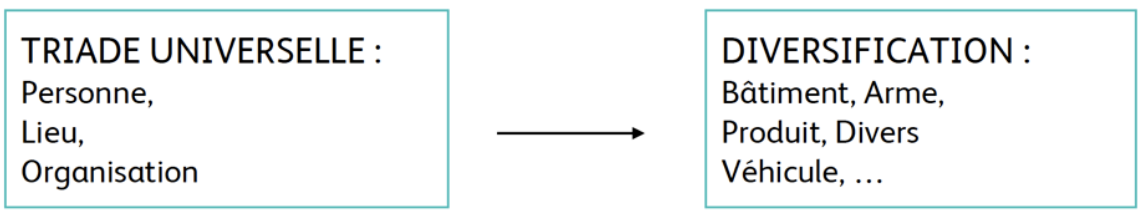
\includegraphics[width=1\linewidth]{img/categorisation.png}
			\caption{Le choix des catégories des \textsc{EN}.}
			\label{fig:ling_out_TAL}
		\end{figure}

					\begin{figure}[h] % Use [H] to force the figure to stay in place
			\centering
			
\includegraphics[width=1\linewidth]{img/couverture.png}
					\caption{La détermination de ce que les \textsc{EN} recouvrent.}
			\label{fig:ling_out_TAL}
		\end{figure}

	
	$\rightarrow$ \textcolor{deepred}{catégorisation instable}
\end{frame}

\begin{frame}{Les \textsc{EN} dans le texte : le problème de l'annotation}
	\begin{itemize}
		\item \textcolor{deepblue}{\textbf{Combinaisions de syntagmes : une ou plusieurs entités ?}}
		\begin{itemize}
			\item \textit{Les banques centrales américaine et européenne ont décidé$\dots$}
			\item 	\textit{Donald et Melania Trump}
			\item \textit{l'université de Genève}
		\end{itemize}
		\item \textcolor{deepblue}{\textbf{Un syntagme : quelles frontières ?}} 
		\begin{itemize}
			\item \textit{la candidate Ségolène Royal, Professeur Paolucci}
			\item \textit{George W. Bush Jr.}, \textit{La Mecque}, \textit{l'Abbé Pierre}
		\end{itemize}
		\item \textcolor{deepblue}{\textbf{Une entité : quelle unité lexicale ?}} 
		\begin{itemize}
			\item 		\textit{Émmanuel Macron}, \textit{Monsieur Macron}, \textit{le Président Émmanuel Macron}, \textit{le Président français}, \textit{le Président de la République française}, \textit{Manu}
		\end{itemize}

	\end{itemize}
	
	$\rightarrow$ \textcolor{deepred}{caractérisation imprécise, diversité des mentions}
\end{frame}

\begin{frame}{Les \textsc{EN} dans la langue : le problème des polysémies}
	\begin{itemize}
		\item \textcolor{deepblue}{\textbf{Homonymie}}
		\begin{itemize}
			\item \textit{Orange a invité M. \underline{Hollande}}
		\end{itemize}
		\item \textcolor{deepblue}{\textbf{Métonymie}}
		\begin{itemize}
			\item \textit{\underline{Leclerc} a fermé ses magasins en Rhône-Alpes}
		\end{itemize}
		\item \textcolor{deepblue}{\textbf{\og{}Facettes\fg{}}}
		\begin{itemize}
			\item \textit{\underline{Le candidat Sarkozy}, devenu \underline{chef de l'État}, a changé de position sur la présence française au sein de la force internationale.}
		\end{itemize}
		
		$\rightarrow$ \textcolor{deepred}{polyréférentialité}
	\end{itemize}
\end{frame}

\begin{frame}{\textsc{EN} : un objet \textsc{TAL} difficile à cerner}
	\begin{itemize}
	\item 	\textcolor{deepblue}{\textbf{Hétérogénéité des réalisations}}
	\begin{itemize}
		\item Les \textsc{EN} ne se limitent pas à une catégorisation, une mention, une interprétation
	\end{itemize}
		\item \textcolor{deepblue}{\textbf{Hétérogénéité des points de vue}}
		\begin{itemize}
			\item formules définitoires sous la forme d'énumérations
			\item caractérisation diverses (sens, forme)
		\end{itemize}
		\end{itemize}
		
		$\rightarrow$ \textcolor{deepred}{Question : que sont les \textsc{EN} ?}
\end{frame}

\begin{frame}{Le \og{}matériau\fg{} de départ}
	 
			\begin{figure}[h] % Use [H] to force the figure to stay in place
			\centering
			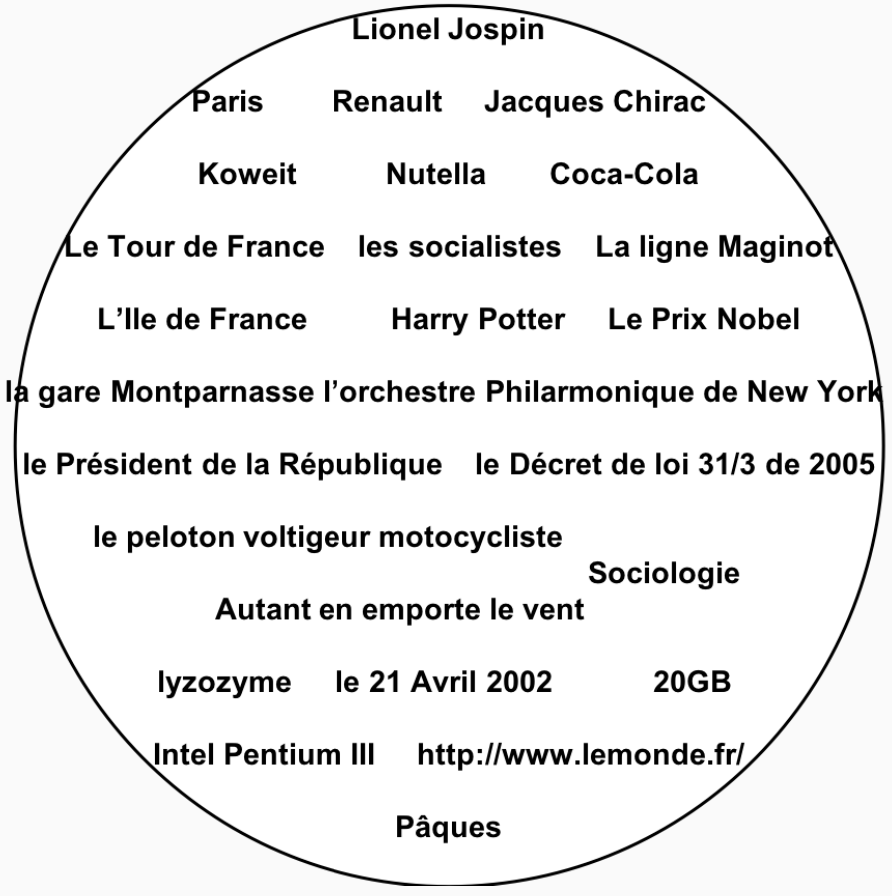
\includegraphics[width=.6\linewidth]{img/materiau_depart.png}
			\label{fig:ling_out_TAL}
			\caption{Unités lexicales considérées comme des \textsc{EN}.}
		\end{figure}

\end{frame}

\begin{frame}{Le \og{}matériau de départ\fg{}}
				\begin{figure}[h] % Use [H] to force the figure to stay in place
		\centering
		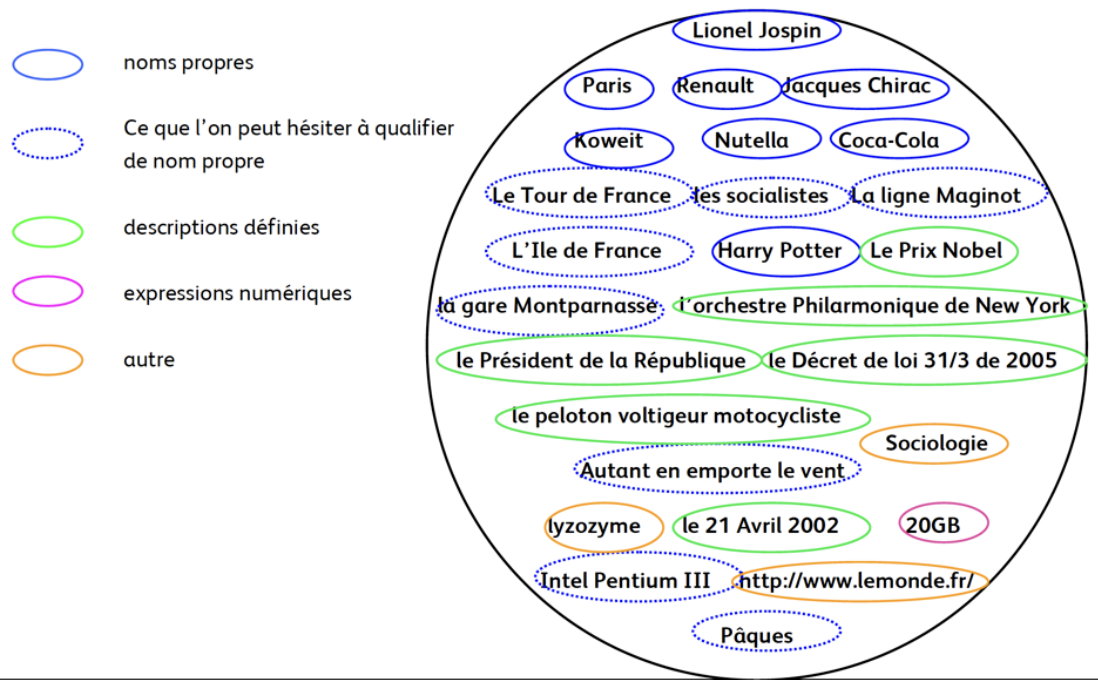
\includegraphics[width=1\linewidth]{img/materiau_depart2.png}
		\caption{Proposition de catégorisation des \textsc{EN}.}
		\label{fig:ling_out_TAL}
	\end{figure}
\end{frame}



\begin{frame}{Unicité référentielle}
	\begin{itemize}
		\item \bolder{Le nom propre se réfère à un particulier}
		\begin{itemize}
			\item \textcolor{deepblue}{\textbf{nomination d'un particulier}} : \textit{Felix} \textit{vs.} nomination d'une classe conceptuelle (\textit{chat})
			\item \textcolor{deepblue}{\textbf{unicité}} : une individualité considérée comme unique au sein d'une catégorie d'existants
			\item \textcolor{deepblue}{\textbf{unité}} : une individualité considérée comme formant un tout reconnaissable
		\end{itemize} 
		\item Les descriptions définies
		\begin{itemize}
			\item présupposition d'existence et d'unicité
			\item \textit{le président de la République}, \textit{le père de Charles II}, \textit{le marronnier}\\
			Une description de la forme \og{}le tel et tel\fg{} présuppose qu'il existe une et une seule entité qui soit telle et telle
		\end{itemize}
	\end{itemize}
\end{frame}

\begin{frame}{Autonomie référentielle}
	\begin{block}{\vspace{-0.6cm}}
		\justifying Comment s'opère la référence à une entité unique ?
	\end{block}
	
	
	\textcolor{deepblue}{\textbf{Noms propres}}
	\begin{itemize}
		\item sens instructionnel dénominatif $\rightarrow$ connaissance d'une convention
		\item dénomination non contingente $\rightarrow$ désignateur rigide
		\item dénomination plus ou moins descriptive (\textit{Massif Central})
	\end{itemize}
	
	\textcolor{deepblue}{\textbf{Descriptions définies}}
	\begin{itemize}
		\item sens descriptif
		\item descriptions définies (in)complètes
		\begin{itemize}
			\item \textit{le président}, \textit{le président de la République française en 2003}
		\end{itemize}
	\end{itemize}
\end{frame}

\begin{frame}{Caractérisation linguistique des \textsc{EN}}
	\begin{itemize}
		\item L'ensemble \textsc{EN} n'est pas réductible à une catégorie linguistique
		\begin{itemize}
			\item plus que les noms propres et moins que les descriptions définies
			\end{itemize}
			\item Caractérisation d'un comportement référentiel
			\begin{itemize}
				\item référence à une entité unique et autonomie référentielle
				\begin{itemize}
					\item \textit{Jacques Chirac}, \textit{le Président de la République}, \textit{le costume bleu du président}
				\end{itemize}
			\end{itemize}
	\end{itemize}
	$\rightarrow$ \textcolor{deepred}{La perspective linguistique ne suffit pas}
\end{frame}

\begin{frame}{Proposition de définition}
	\begin{block}{Entité nommée}
		\justifying
		Étant donné un \textcolor{OliveGreen}{modèle applicatif} et un \textcolor{OliveGreen}{corpus}, on appelle entité nommée toute \textcolor{deepred}{expression linguistique} qui \textcolor{deepred}{se réfère} à une \textcolor{deepred}{entité unique} du modèle de manière \textcolor{deepred}{autonome} \textcolor{OliveGreen}{dans le corpus}.
	\end{block}
	
	Questions que l'on s'est posées : 
	\begin{itemize}
		\item Comment définir un objet \textsc{TAL} ?
		\item Que sont les noms propres et les descriptions définies ?
		\item Que devient le cadre linguistique du sens et de la référence en \textsc{TAL} ?
	\end{itemize}
\end{frame}

\begin{frame}{Illustration}
					\begin{figure}[h] % Use [H] to force the figure to stay in place
		\centering
		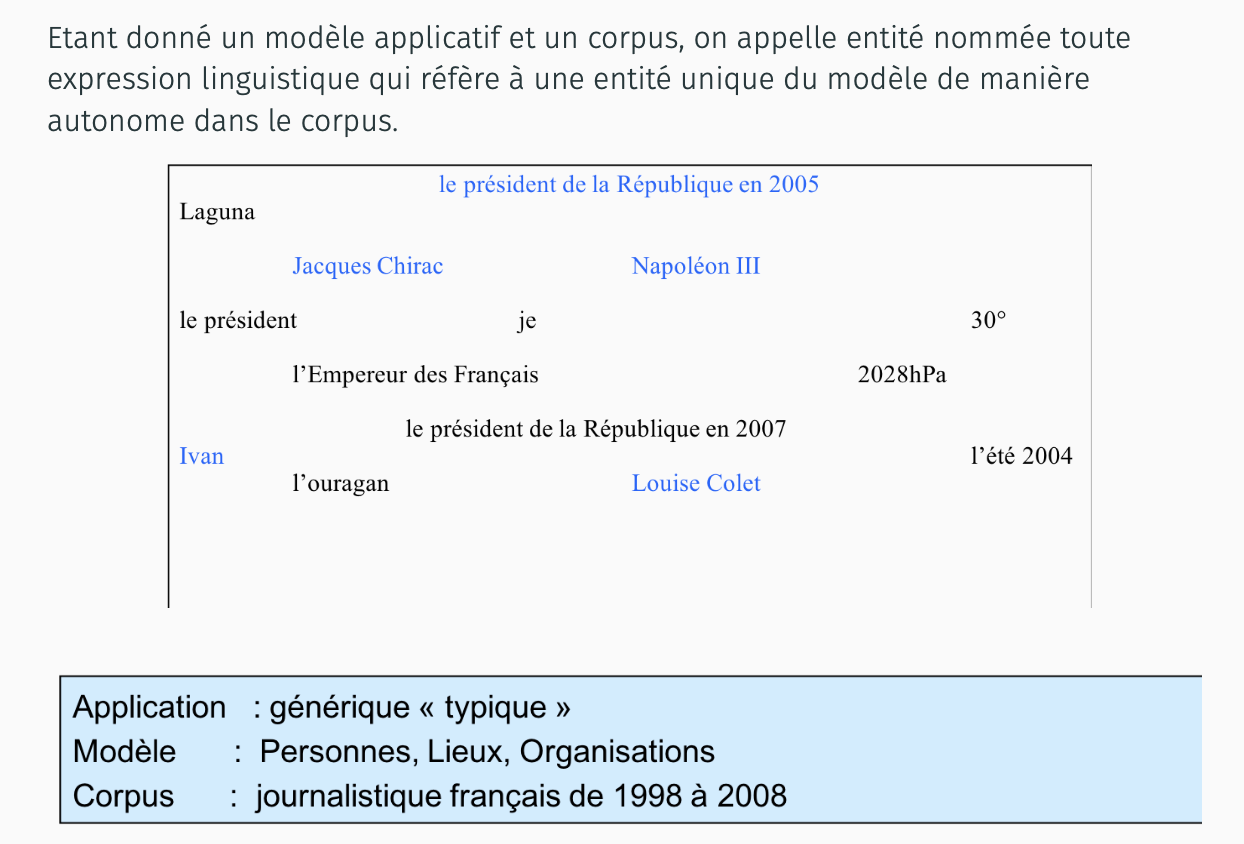
\includegraphics[width=.9\linewidth]{img/generique.png}
		\caption{Cas de figure \textsc{I}.}
		\label{fig:ling_out_TAL}
	\end{figure}
\end{frame}

\begin{frame}{Illustration}
						\begin{figure}[h] % Use [H] to force the figure to stay in place
		\centering
		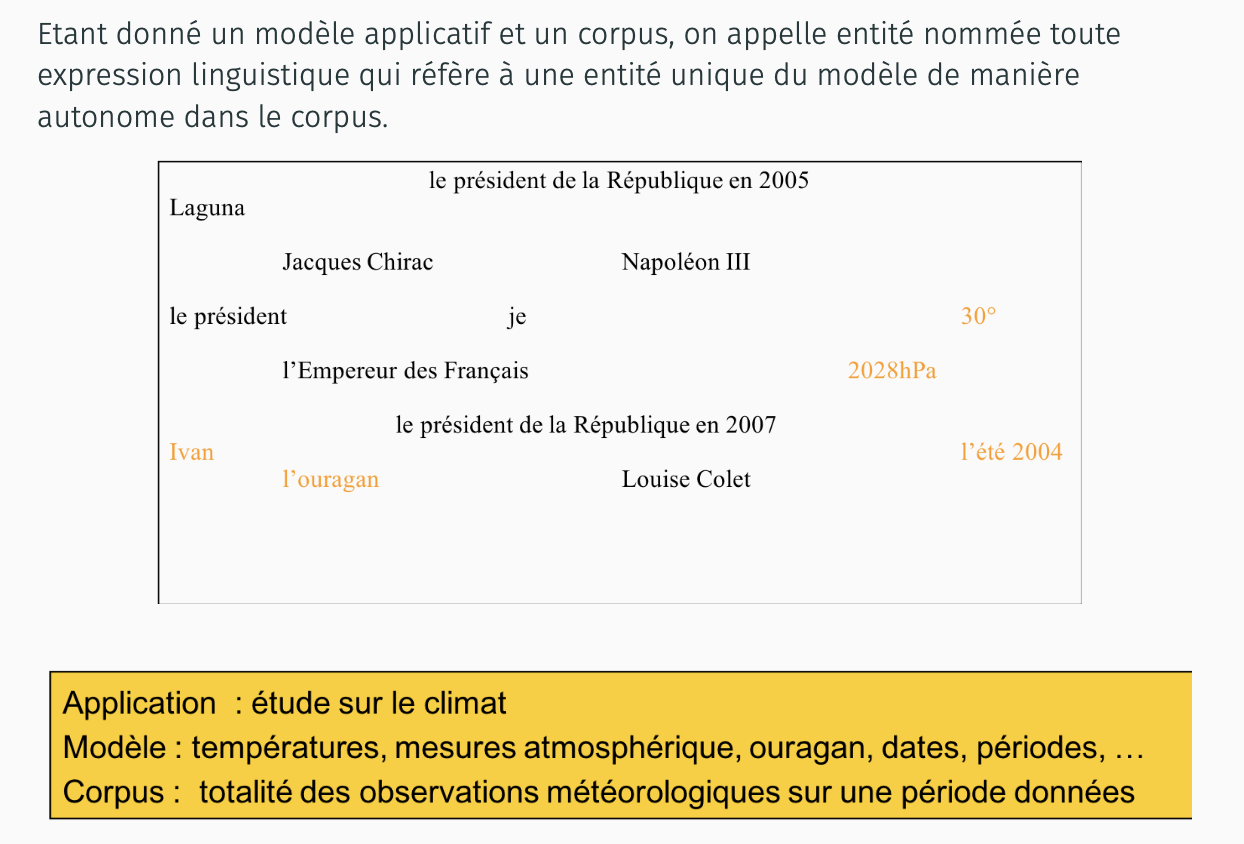
\includegraphics[width=.9\linewidth]{img/climat.png}
		\caption{Cas de figure \textsc{II}.}
		\label{fig:ling_out_TAL}
	\end{figure}
\end{frame}

\begin{frame}{Illustration}
						\begin{figure}[h] % Use [H] to force the figure to stay in place
		\centering
		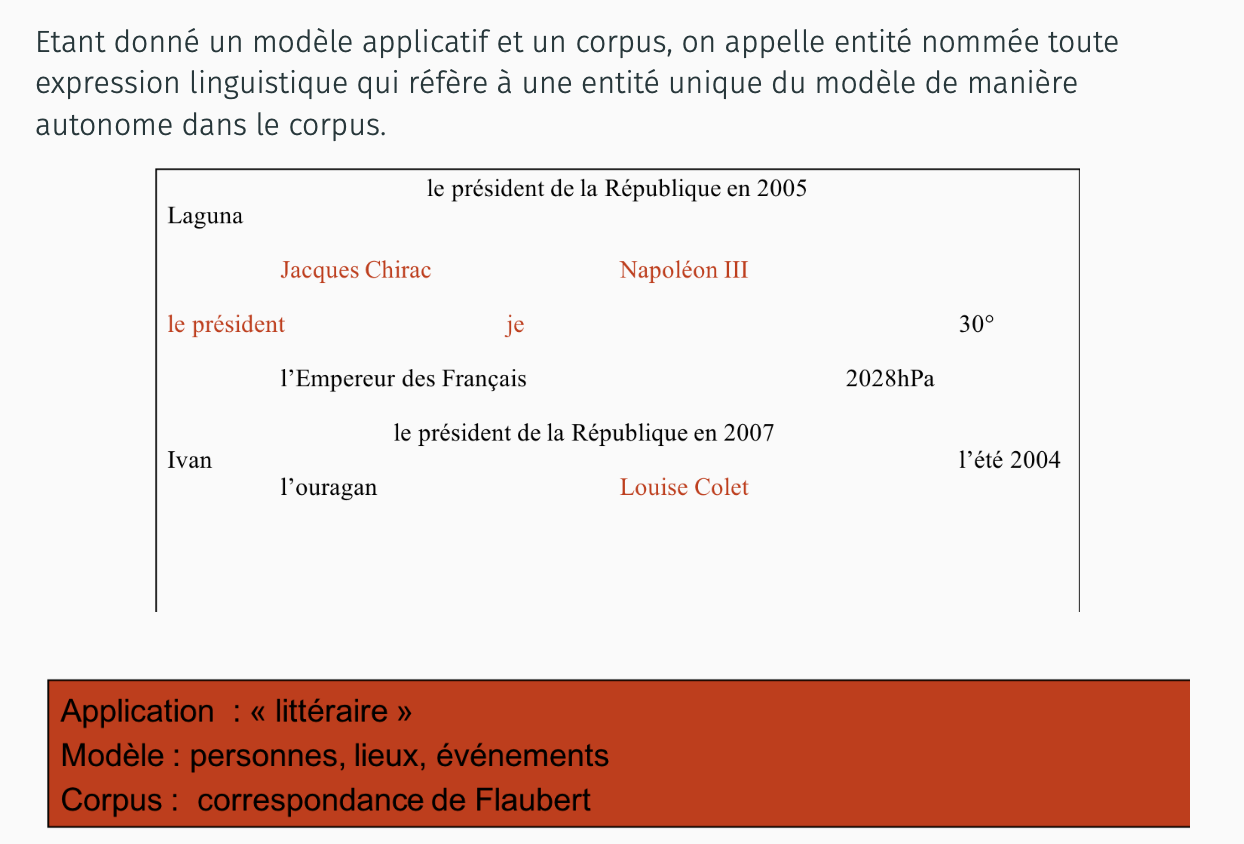
\includegraphics[width=.9\linewidth]{img/litteraire.png}
		\caption{Cas de figure \textsc{III}.}
		\label{fig:ling_out_TAL}
	\end{figure}
\end{frame}

\begin{frame}{Les \textsc{EN} : une création \textsc{TAL}}
	\textcolor{deepblue}{\textbf{De la linguistique au \textsc{TAL}, spécification d'un cadre théorique pour les \textsc{EN}}} :
	\begin{itemize}
		\item perspective linguistique : non réductibles à une catégorie mais caractérisables par un comportement référentiel
		\item perspective \textsc{TAL} : existent relativement à un modèle applicatif précis
	\end{itemize}
	$\rightarrow$ pas d'\textsc{EN} \textit{per se}, seulement des critères linguistiques et un modèle
	
	\textcolor{deepblue}{\textbf{Conséquences : points de vue}}
	\begin{itemize}
		\item général : explication de l'hétérogénéité et de la variabilité de l'ensemble \textsc{EN}
		\item pratique : critères de décision pour annoter
		\item méthodologique : besoin impératif d'expliciter le modèle
	\end{itemize}
\end{frame}

\section{Ressources}

\begin{frame}{Ressources}
	\begin{block}{\vspace{-0.6cm}}
		\justifying
		De quoi a-t-on besoin pour traiter les \textsc{EN} ?
	\end{block}
	
	\begin{enumerate}
		\item \textcolor{deepblue}{\textbf{Typologies}}, pour définir un cadre sémantique
		\item \textcolor{deepblue}{\textbf{Corpus annotés}}, pour servir de référence (évaluation) et d'illustration
		\item \textcolor{deepblue}{\textbf{Lexique et bases de connaissances}}, pour donner des informations sur les éléments à traiter (entraînement)
	\end{enumerate}
\end{frame}

\begin{frame}{Typologie : une façon de structurer}
	Une typologie (angl. \textit{tagset}) est une \textcolor{deepred}{formalisation descriptive} des catégories d'\textsc{EN} à prendre en compte :
	\begin{itemize}
		\item quoi reconnaître (cibler des éléments appartenant à des catégories spécifiques)
		\item comment le représenter (pour un élément, choisir une catégorie parmi d'autres)
	\end{itemize}
	
	De \textcolor{deepred}{multiples variations} en fonction des domaines et des applications -- différences de :
	\begin{itemize}
		\item catégories
		\item structure
		\item sur la définition de ce que recouvrent les catégories
	\end{itemize}
\end{frame}

\begin{frame}{Typologie \textsc{MUC}}
	\begin{itemize}
		\item \textcolor{deepblue}{\textbf{noms propres}} (\textsc{ENAMEX}) : lieux, personnes, organisations
		\item \textcolor{deepblue}{\textbf{expressions numériques}} (\textsc{NUMEX}) : dates et heures (expressions absolues), montants monétaires et pourcentages
	\end{itemize}
	
	\begin{table}[h]
		\centering
		\scriptsize
		\begin{tabularx}{\textwidth}{|X|X|X|}
			\hline
			\multicolumn{1}{|c}{Types} & \multicolumn{1}{|c|}{Exemple} & \multicolumn{1}{c|}{Contre-exemple} \\ \hline		
			\textsc{ORG} &  \textbf{DARPA} & our university\\
			\textsc{PERS}& \textbf{Harry Schearer} & St. Michael \\
			\textsc{LOC} & \textbf{\textsc{U.S}}. & 53140 Gatchell Road\\
			\hline
			\textsc{MONEY}& \textbf{19 dollars} & ça en coûte 19 \\
			\textsc{TIME} & \textbf{8 heures} & la nuit dernière \\
			\textsc{DATE} & en \textbf{juillet} & en \textbf{juillet} dernier\\
			\hline
		\end{tabularx}
		\caption{Le qualitatif : données, informations et connaissances.}
	\end{table}
	
\end{frame}

\begin{frame}{Typologie \textsc{ACE}}
		\begin{table}[h]
		\centering
		\scriptsize
		\begin{tabularx}{\textwidth}{|X|X|}
			\hline
			\multicolumn{1}{|c}{\textbf{Types}} & \multicolumn{1}{|c|}{\textbf{Sous-types}} \\
			\hline
			\textsc{PERS} & individu, groupe, indéterminé \\ \hline
			\textsc{ORG} & (non) gouvernementales, commerciales, éducation, divertissement, média, religieuses, médicales, sciences, sports \\
			\hline
			\textsc{GPE} & continent, nation, état ou province, département ou région, villes, groupement de \textsc{GPE}, spécial, ainsi que des types comme \textsc{PERS}, \textsc{LOC}, \textsc{ORG} \\
			\hline
			\textsc{LOC} & adresses, frontières, objets astronomiques, plans d'eau, région géographique, région internationale, autre\\
			\hline
			\textsc{FAC} & aéroports, usines, constructions, portion de construction\\
			\hline
			\textsc{VEH} & air, terre, eau, portions de véhicule, non spécifié\\
			\hline
			\textsc{WEA} & contondantes, explosives, coupantes, chimiques, biologiques, armes à feu, munitions, nucléaires, non spécifiées\\
			\hline
		\end{tabularx}
		\caption{Le qualitatif : données, informations et connaissances.}
	\end{table}
\end{frame}

\begin{frame}{Évolution}
	Nombreuses autres typologies s'inspirant de \textsc{MUC} et \textsc{ACE}
	\begin{itemize}
		\item \textsc{CoNLL} : inspiration \textsc{MUC}, ajout d'une catégorie \textsc{misc}
		\item \textsc{HAREM} : inspiration \textsc{ACE}, ajout de différentes catégories (\textsc{Idée}, \textsc{Objet}, \textsc{Autre}, \textsc{Groupe})
		\item \textsc{ESTER-2} : encore plus de sous-types (\textsc{pers.hum}, \textsc{pers.anim}, \textsc{loc.geo}, \textsc{loc.admin} etc.) et traitement de l'imbrication
	\end{itemize}
\end{frame}

\begin{frame}{Imbrication des \textsc{EN}}
	Au-delà de la structuration en type et sous-types, il y a la notion de l'imbrication :
	\begin{itemize}
		\item une entité peut en contenir une autre
		\item \textit{The \texttt{<pers>} president of \texttt{<org>} Ford \texttt{</org>} \texttt{</pers>}}
	\end{itemize}
	
	Structuration très utilisée dans des domaines de spécialité, p. ex. la typologie \textsc{GENIA} (domaine bio-médical)
\end{frame}

\begin{frame}{La typologie \textsc{QUAERO}}
	\begin{enumerate}
		\item \textcolor{deepblue}{\textbf{Personne}} : personne individuelle, groupe de personnes
		\item \textcolor{deepblue}{\textbf{Lieu}} : lieu administratif, lieu physique, construction, odonyme, adresse
		\item \textcolor{deepblue}{\textbf{Organisation}} : administration, service
		\item \textcolor{deepblue}{\textbf{Expression temporelle}} : date / heure absolue et relative
		\item \textcolor{deepblue}{\textbf{Montant}}
		\item \textcolor{deepblue}{\textbf{Produit}} : objet manufacturé, route, produit financier, doctrine, loi, \textit{software}, art, média, récompense
		\item \textcolor{deepblue}{\textbf{Fonction}} : individuelle ou collective
	\end{enumerate}
\end{frame}

\begin{frame}{Typologie \textsc{QUAERO} : sous-types}
							\begin{figure}[h] % Use [H] to force the figure to stay in place
		\centering
		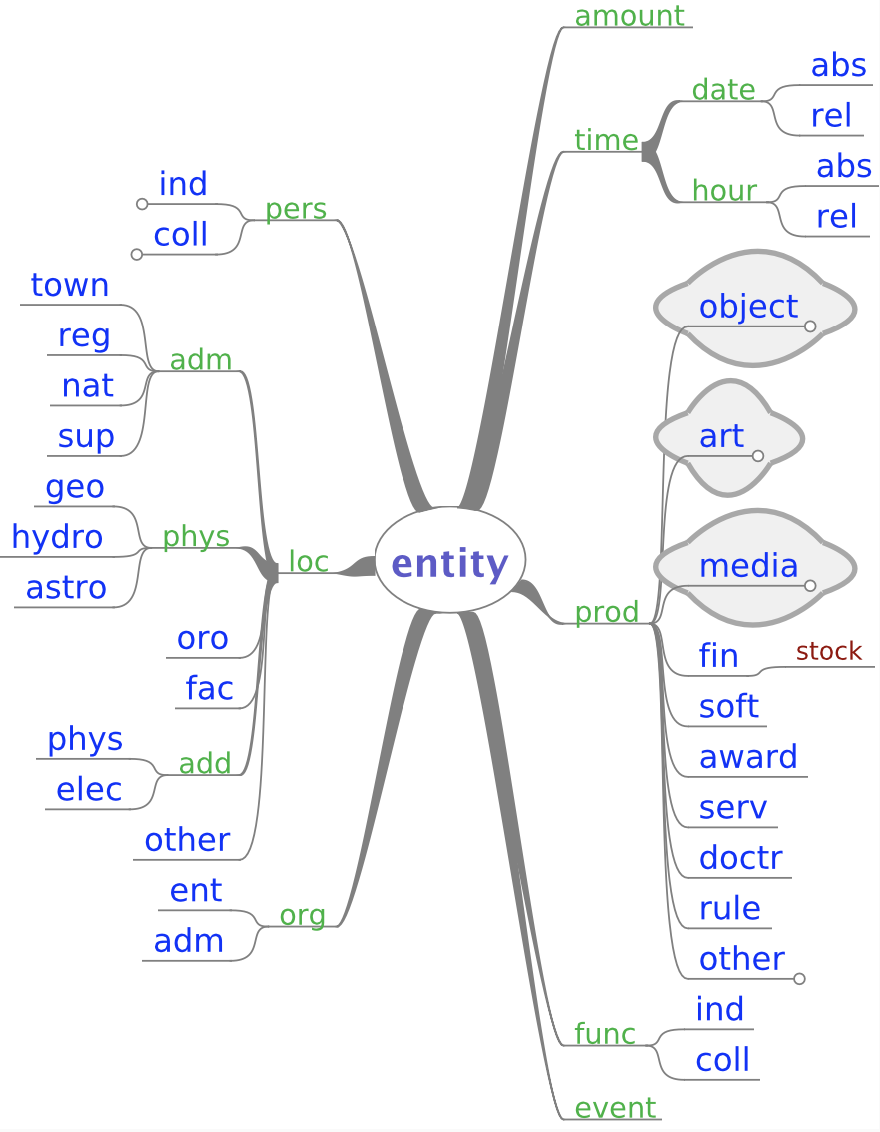
\includegraphics[width=.5\linewidth]{img/quaero_sous-types.png}
		\caption{Les sous-types de la typologie \textsc{QUAERO}.}
		\label{fig:ling_out_TAL}
	\end{figure}
\end{frame}

\begin{frame}{Typologie \textsc{QUAERO} : composants d'entités}
		\begin{figure}[h] % Use [H] to force the figure to stay in place
		\centering
		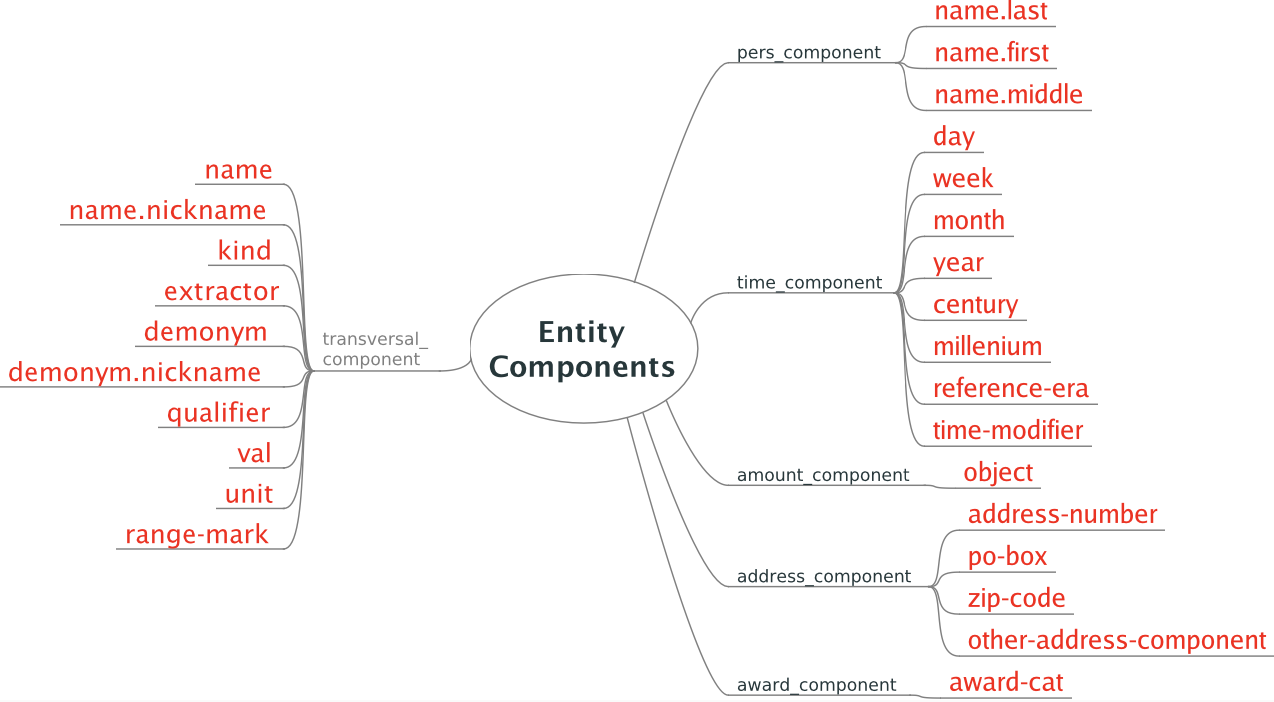
\includegraphics[width=1\linewidth]{img/quaero_composants_entites.png}
		\caption{Les composants d'entités de la typologie \textsc{QUAERO}.}
		\label{fig:ling_out_TAL}
	\end{figure}
\end{frame}

\begin{frame}{\textsc{QUAERO} : composants d'entités}
			\begin{figure}[h] % Use [H] to force the figure to stay in place
		\centering
		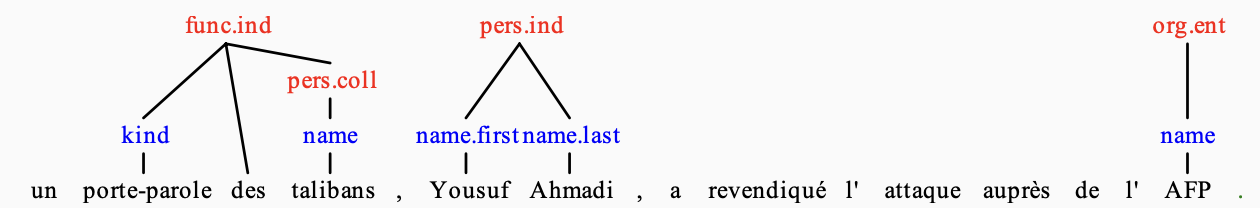
\includegraphics[width=1\linewidth]{img/quaero_composants_entites_2.png}
		\caption{Les composants d'entités de la typologie \textsc{QUAERO}.}
		\label{fig:ling_out_TAL}
	\end{figure}
	
	Les composants permettent : 
	\begin{itemize}
		\item d'avoir, par compositionnalité, de nombreux types sans les multiplier
		\item d'aider au suivi et à la liaison, au moins \textit{intra}-documents (\textit{l'usine Renault} $\rightarrow$ \textit{l'usine})
	\end{itemize}
\end{frame}

\begin{frame}{Comparaison de typologies par l'exemple}
			\begin{table}[h]
		\centering
		\scriptsize
\resizebox{1\textwidth}{!}{
		\begin{tabularx}{\textwidth}{|p{0.7cm}|X|}
			\hline
			\textsc{MUC} & d'après le Bureau du recensement des \bolder{LOC}\colorbox{Cerulean!30}{[\textit{États-Unis}]}, les revenus des ménages ont reculé pour la quatrième année consécutive en \bolder{DATE}\colorbox{Cerulean!30}{[\textit{2011}]}. \\
			\hline
			\textsc{ACE} & d'après le \bolder{ORG}\colorbox{Cerulean!30}{[\textit{Bureau du recensement des États-Unis}]}, les revenus des ménages ont reculé pour la quatrième année consécutive en \bolder{DATE}\colorbox{Cerulean!30}{[\textit{2011}]}.\\
			\hline
			\textsc{EST} & d'après le \bolder{ORG}\colorbox{Cerulean!30}{[\textit{Bureau du recensement des} \bolder{LOC} [\textit{États-Unis}]]}, les revenus des ménages ont reculé pour la quatrième année consécutive en \bolder{DATE}\colorbox{Cerulean!30}{[\textit{2011}]}.\\
			\hline
			\textsc{QUA} & d'après le \bolder{ORG} [\colorbox{Cerulean!30}{\textcolor{deepred}{name} [\textit{Bureau du recensement}] \textit{des} \bolder{LOC} [\textcolor{deepred}{name}  [\textit{États-Unis}]]}, les revenus des ménages ont reculé pour la quatrième année consécutive en \bolder{DATE}\colorbox{Cerulean!30}{[\textcolor{deepred}{year} [\textit{2011}]]}.\\
			\hline
		\end{tabularx}
	}
		\caption{Comparaison de typologies des \textsc{EN}.}
	\end{table}
\end{frame}

\begin{frame}{\textit{Text Analysis Conference -- Knowledge Base Population}}
	Pour une \textsc{EN} donnée, il importe de trouver de nombreux attributs.
	P. ex. pour une entité de type \textsc{PERS} : 
	\begin{itemize}
		\item noms : les autres noms que porte ou a porté cette personne (\textit{alias}, faux noms, noms de scène, etc.)
		\item fonctions et activités : ses emplois, ses occupations, etc.
		\item dates (ou âge) : de naissance, de mort, des différents évènements, son âge
		\item lieux : en rapport avec des évènements de sa vie comme la naissance, la mort, les différents emplois, etc.
		\item personnes liées : conjoint(e), enfants, autres membres de sa famille, etc.
		\item autres informations : écoles et universités fréquentées, pays visités, etc.
	\end{itemize}
	
	$\rightarrow$ retour à la compréhension
\end{frame}

\begin{frame}{Corpus annoté et guide d'annotation}
	\begin{block}{\vspace{-0.6cm}}
		\justifying
		Un \textcolor{deepred}{ensemble de documents textuels} dont le texte est enrichi, lors d'une \textcolor{deepred}{campagne d'annotation}, par un \textcolor{deepred}{marquage} des \textsc{EN} respectant une \textcolor{deepred}{typologie} donnée.
	\end{block}
	
	Typologie $\rightarrow$ manuel d'annotation
\begin{itemize}
	\item exemplification des catégories
	\item règles pour permettre à l'annotateur de faire des choix
	\item souvent, définition en parallèle de la typologie et de guide d'annotation
\end{itemize}
\end{frame}

\begin{frame}{Campagne d'annotation}
	\begin{itemize}
		\item à partir d'outils dédiés (\textsc{brat}\footnote{\url{https://brat.nlplab.org/introduction.html}}, \textsc{Glozz}\footnote{\url{http://explorationdecorpus.corpusecrits.huma-num.fr/glozz/}}, \textsc{WebAnno}\footnote{\url{https://webanno.github.io/webanno/}})
		\item importance de la mesure de la qualité et de la cohérence des annotations
		\item publication du corpus avec des informations : sources, accord inter-annotateur, mesures utilisées, typologie et guide d'annotation
		\item à faire avec soin : chronophage et gourmand en ressources
	\end{itemize}
	
	Exemples de corpus français : \textsc{ESTER 2}, \textsc{QUAERO}, \textsc{ETAPE}

\end{frame}

\begin{frame}{Lexiques et bases de connaissances}
	Objectif : \textcolor{deepred}{fournir des informations relatives à des \textsc{EN}}, en général ou dans des domaines de spécialité, sur lesquelles les \textcolor{deepred}{systèmes automatiques peuvent s'appuyer} afin de les reconnaître, les catégoriser et les désambiguïser.
	
	Types d'informations : 
	\begin{enumerate}
		\item lexicales, sur les unités composant les \textsc{EN}
		\item encyclopédiques, sur les référents des \textsc{EN}
	\end{enumerate}
	
%	Élément central pour la reconnaissance et la classification des \textsc{EN} (mais évolution avec l'apprentissage profond)
%	
		Évolution importante de ce type de ressource depuis l'apparition de la tâche :
	\bolder{index géographiques} (angl. \textit{gazetteers}) $\rightarrow$ encodage de plus en plus d'information
\end{frame}



\begin{frame}{Bases lexicales}
		Encodent 2 types d'information : 
	\begin{itemize}
		\item des \textcolor{deepblue}{\textbf{noms ou parties de noms d'entités}} avec leurs types associés, p. ex. \textit{Justin}
		$\rightarrow$ directement utilisés pour reconnaître des unités équivalentes dans les textes		
		\item des \textcolor{deepblue}{\textbf{mots amorces}}, également avec leurs types associés, p. ex. \textit{Monsieur}
		$\rightarrow$ des unités indiquant avec une forte probabilité la présence d'une \textsc{EN} d'un certain typye
	\end{itemize}
	\begin{itemize}
		\item \textsc{WordNet}\footnote{\url{https://wordnet.princeton.edu/}} : utile pour l'intégration de ressources
		\item \textsc{PROLEX}\footnote{\url{https://www.ortolang.fr/market/lexicons/prolex}} : base d'\textsc{EN} multilingue
		\item \textsc{Geonames}\footnote{\url{https://www.geonames.org/}} : toponymes et assimilés
	\end{itemize}
\end{frame}

\section{Reconnaissance et classification}
\begin{frame}{Objectifs}
	Construire des systèmes logiciels qui effectuent ces tâches de manière automatique.
	
	Exigences : 
	\begin{itemize}
		\item \bolder{qualité} : ne pas faire trop d'erreurs
		\item \bolder{exhaustivité} : ne pas manquer trop d'\textsc{EN}
		\item \bolder{robustesse} : ne pas échouer face à des cas non canoniques
	\end{itemize}
	
	En pratique : 
	\begin{itemize}
		\item difficile de répondre à ces exigences simultanément
		\item recherche du \textcolor{deepblue}{\textbf{meilleur compromis}} en fonction des ressources et de l'application
	\end{itemize}
\end{frame}

\begin{frame}{Représentation du texte}
	La représentation des textes comme séquences de mots donne 2 niveaux de granularité : 
	\begin{itemize}
		\item \textbf{caractères}, qui forment un mot
		\item \textbf{mots}, qui composent une séquence (un texte)
	\end{itemize}
	
	Les \bolder{indices} peuvent être caractérisés au niveau : \begin{itemize}
		\item des caractères : \textcolor{deepblue}{\textbf{indices morphologiques}}
		\begin{itemize}
			\item majuscule, régularités socio-culturelles (\textit{-ville}), nombres
		\end{itemize}
		\item des mots eux-mêmes : \textcolor{deepblue}{\textbf{indices lexicaux}}
				\begin{itemize}
			\item confronter les textes à des listes d'\textsc{EN} de composants d'\textsc{EN}
		\end{itemize}
		\item de la séquence de mots : \textcolor{deepblue}{\textbf{indices contextuels}}
				\begin{itemize}
			\item contextes local (mots qui précèdent ou suivent l'\textsc{EN}) et global (phrase(s), etc.)
		\end{itemize}
	\end{itemize}
\end{frame}

\begin{frame}{Approches symboliques}
	\bolder{Techniques à base d'automates}
	
	\begin{itemize}
		\item insertion de balises dans les textes indiquant où se trouvent les \textsc{EN}
		\item conception de \textcolor{deepblue}{\textbf{règles}} formant une \textcolor{deepblue}{\textbf{grammaire locale}}
		\item boîtes à outils : Unitex, \textsc{GATE}, \textsc{NooJ}, etc.
	\end{itemize}
	
	Pré-traitements : segmentation en mots, en phrases, étiquetage morphosyntaxique
	
	
	$\rightarrow$ indices supplémentaires fort utiles, mais qui impactent les performances si bruités
\end{frame}

\begin{frame}{Approches statistiques}
	Au début des années 2000, grâce à la mise à disposition de jeux de données volumineux.
	
	Mais les approches symboliques sont toujours présentes : 
	\begin{itemize}
		\item combinées avec des méthodes statistiques
		\item prédominent pour les langues ou les typologies sans corpus de données suffisants
		\item gardent l'atout pour le contrôle et de l'ingénierie : plus compréhensibles, modulables, possibilités de réglages fins
		\item majoritaires dans le milieu industriel
		\end{itemize}
\end{frame}

\begin{frame}{Apprentissage automatique}
	Modèles \bolder{guidés par les données} (angl. \textit{data-driven} models)
	
	Objectif : déterminer les paramètres d'un modèle à partir de données, d'où le terme \bolder{apprentissage}
	
	Ces paramètres et ce modèle sont ensuite utilisés pour prendre les décisions les plus probables (ou vraisemblables) sur de nouvelles données à traiter.
	
	Il s'agit, simultanément, de spécifier le modèle et de généraliser sur les données.
\end{frame}

\begin{frame}{Le paradigme de l'apprentissage automatique}
	\bolder{Systèmes symboliqes} : le concepteur du système interagit majoritairement avec le modèle (l'automate), et n'utilise les données que pour visualiser ou pour évaluer
	
	\bolder{Systèmes guidés par les données} : le concepteur agit sur les données, la structure du modèle est prédéfinie et rigide et les paramètres ajustés automatiquement à partir des données.
	
				\begin{figure}[h] % Use [H] to force the figure to stay in place
		\centering
		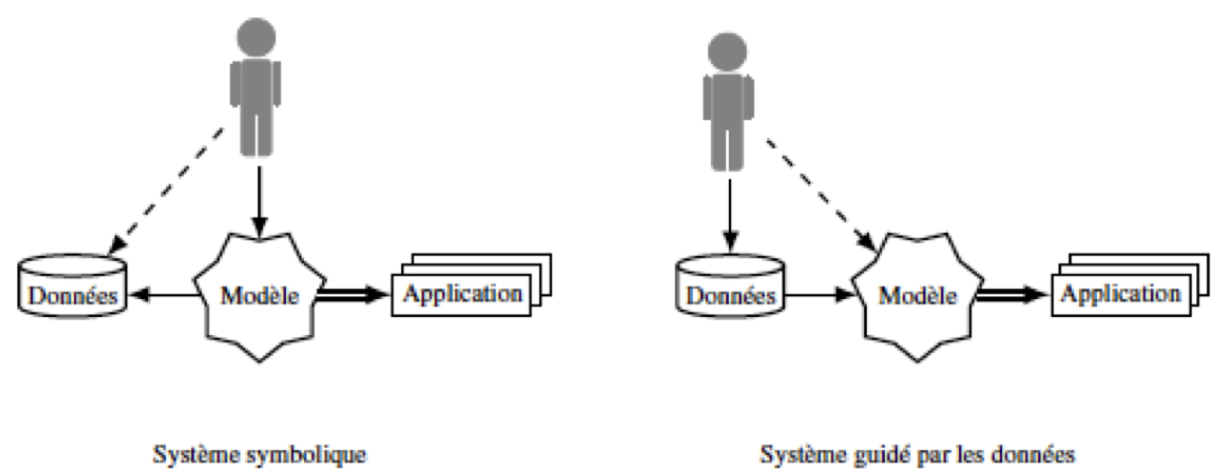
\includegraphics[width=.7\linewidth]{img/paradigme_apprentissage.png}
		\caption{Système symbolique \textit{vs.} système guidé par les données.}
		\label{fig:ling_out_TAL}
	\end{figure}
\end{frame}

\begin{frame}{Approches existantes}
	La \textsc{REN} peut être formalisée comme une tâche de \bolder{classification}.
	
	\begin{itemize}
		\item arbres de décision
		\item modèles probabilistes
		\item réseaux neuronaux
	\end{itemize}
\end{frame}

\begin{frame}{Modèles par classes majoritaires}
	Déterminer la classe d'un mot à partir de la classe qui lui est majoritairement associée dans le corpus d'apprentissage.
	
	Formulation à l'aide des probabilités :
	\begin{itemize}
		\item fréquence du mot $F(m)$
		\item fréquence d'une étiquettee $F(e)$
		\item fréquence de la présence jointe du mot et de l'étiquette $F(m,e)$
		\end{itemize}
\end{frame}

\begin{frame}{Modèles par classes majoritaires}
	La formule de Bayes et l'estimation statistique permettent de calculer la probabilité d'une étiquette étant donné le mot :
	\begin{equation*}
	P(E_{i} = e|M_{i} = m) = \dfrac{P(M_{i} = m, E_{i} = e)}{P(M_{i} = m)} = \dfrac{F(e,m)}{F(m)}
	\end{equation*}
	
	Probabilité d'une étiquette pour un mot donné = ratio entre la fréquence du mot avec une étiquette dans le corpus annoté et la fréquence du mot dans ce même corpus, quelle que soit l'étiquette.
\end{frame}

\begin{frame}{Modèles par classes majoritaires}
					\begin{figure}[h] % Use [H] to force the figure to stay in place
		\centering
		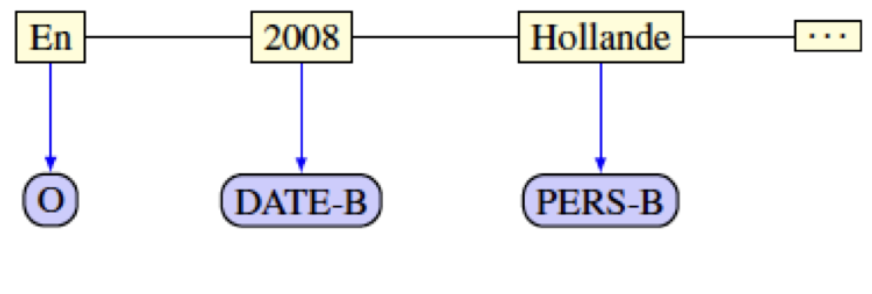
\includegraphics[width=.9\linewidth]{img/classes_majoritaires.png}
		\caption{Modèle par classes majoritaires. L'orientation des flèches indique quelles dépendances sont prises en compte par le modèle.}
		\label{fig:ling_out_TAL}
	\end{figure}
\end{frame}

\begin{frame}{Modèles à décisions contextuelles (\textsc{HMM})}
	Objectif : tenir compte de la vraisemblance d'\bolder{étiquettes contiguës}
	\begin{center}
		\textit{François Hollande}
	\end{center}
	
	\begin{itemize}
		\item \textit{Hollande} : \textsc{Lieu} ou \textsc{Personne} ?
		\item \textit{François} : annoté comme \textsc{Personne}, peut conditionner l'annotation du mot \textit{Hollande}
	\end{itemize}
\end{frame}

\begin{frame}{Modèles à décisions contextuelles (\textsc{HMM})}
	Option : modèles génératifs comme les modèles de Markov à états cachés.
	
	\bolder{Calcul des probabilités inverse} : déterminer, pour une suite d'étiquettes, la probabilité qu'elle génère un texte donné.
	
	\begin{equation*}
		P(M_{1}, M_{2}\dots, M_{n}|E_{1}, E_{2},\dots, E_{n}) = \prod_{i=1}^{n}P(M_{i}|E_{i}) \times P(E_{i}|E_{i-1})
	\end{equation*}
	
	Soit le produit des probabilités de génération $P(M_{i}|E_{i})$ et de transition $P(E_{i}|E_{i-1})$
\end{frame}

\begin{frame}{Modèles à décisions contextuelles (\textsc{HMM})}
						\begin{figure}[h] % Use [H] to force the figure to stay in place
		\centering
		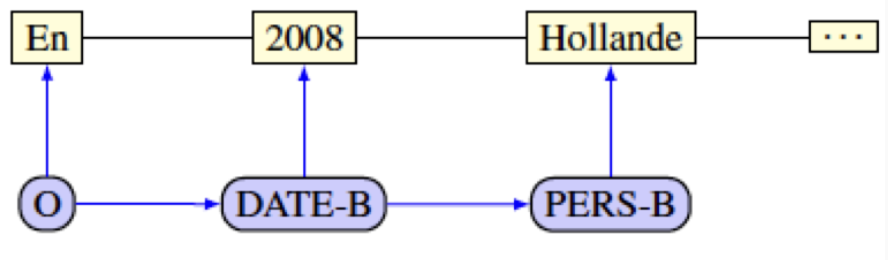
\includegraphics[width=.9\linewidth]{img/hmm.png}
		\caption{Modèle de Markov à états cachés. Décisions non indépendantes : la solution la plus vraisemblable est choisie en fonction des étiquettes préalablement choisies.}
		\label{fig:ling_out_TAL}
	\end{figure}
\end{frame}

\begin{frame}{Modèles utilisant des indices multiples (\textsc{Softmax}, \textsc{MaxEnt})}
	Objectif : \textcolor{deepblue}{\textbf{considérer plus d'indices que les mots}}, \textit{i.e.} prendre en compte la morphologie, les indices lexicaux, le contexte, etc.
							\begin{figure}[h] % Use [H] to force the figure to stay in place
		\centering
		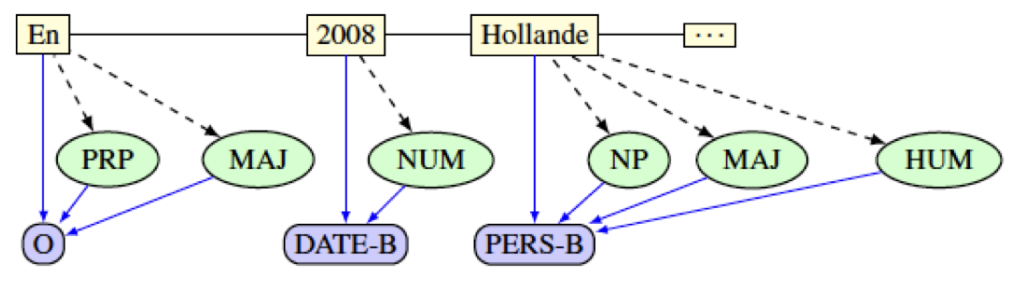
\includegraphics[width=.9\linewidth]{img/indices_multiples.png}
		\caption{Tenir compte d'indice sur les tokens.}
		\label{fig:ling_out_TAL}
	\end{figure}
\end{frame}

\begin{frame}{Champs aléatoires conditionnels (\textsc{CRF})}
	Les \bolder{\textsc{CRF}} (angl. \textit{Conditional Random Fields}) ou champs aléatoires conditionnels combinent les deux aspects précédents : 
	\begin{itemize}
		\item \textcolor{deepblue}{\textbf{tenir compte du contexte}} pour prendre des décisions (une décision sur un mot influence la décision pour le mot suivant)
		\item \textcolor{deepblue}{\textbf{tenir compte de multiples indices}} (analyses en pré-traitements)
	\end{itemize}
\end{frame}

\begin{frame}{Champs aléatoires conditionnels (\textsc{CRF})}
									\begin{figure}[h] % Use [H] to force the figure to stay in place
		\centering
		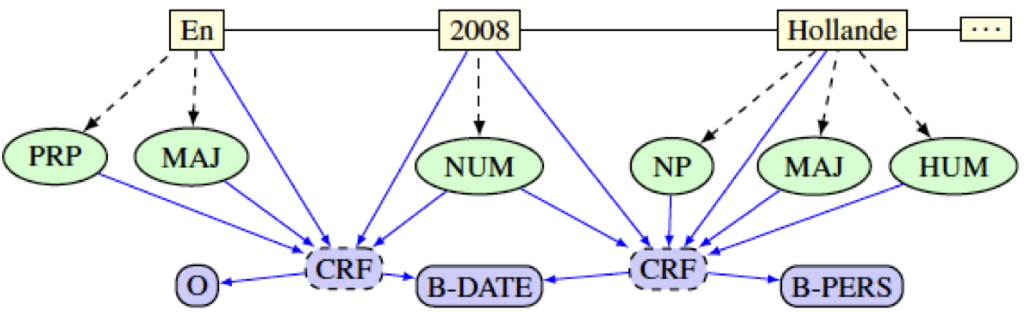
\includegraphics[width=.9\linewidth]{img/crf.png}
		\caption{Modèle graphique \textsc{CRF}.}
		\label{fig:ling_out_TAL}
	\end{figure}
	
	\begin{equation*}
			G(e,m,f_{1},\dots,f_{k}) = \exp \left( \sum_{p=1}^{k} \alpha_{ep} \times f_{p} \right)
	\end{equation*}

Fonction exponentielle pour évaluer la pertinence d’un état donné en fonction d’un ensemble de caractéristiques.
	
\end{frame}

\section{Liaison}

\begin{frame}{Où en sommes-nous ?}
	\begin{itemize}
		\item nous savons reconnaître et catégoriser des segments textuels : des \textcolor{deepblue}{\textbf{mentions}} d'\textsc{EN} qui font référence à un \textcolor{deepblue}{\textbf{objet}} du monde
		\item ce qu'il reste à faire : établir le lien entre les mentions et les objets auxquels elles se réfèrent
	\end{itemize}
	
	$\rightarrow$ objectif : \bolder{désambiguïsation, résolution, liaison}
\end{frame}

\begin{frame}{Des mentions aux référents}
	\textcolor{deepblue}{\textbf{Catégoriser n'est pas désambiguïser}}
	\begin{itemize}
		\item \textit{G. Bush} et \textit{F. Mitterrand} sont des \textsc{Person}
		\item lequel des deux se réfère-t-il au 43\ieme{} président des États-Unis ?
	\end{itemize}
	
	\textcolor{deepblue}{\textbf{Le problème des homonymes}}
	\begin{itemize}
		\item \textit{F. Mitterrand} est une \textsc{Person} (\textit{François} ou \textit{Frédéric} ?)
		\item \textit{Bush} est une \textsc{Person} (\textit{G. Bush} ou \textit{G. W. Bush} ?)
	\end{itemize}
	
	\textcolor{deepblue}{\textbf{Le problème des variantes}} 
	\begin{itemize}
		\item \textit{Jean-Claude Juncker}, \textit{Juncker} et \textit{le président de la Commission Européenne} se réfèrent-elles à la même \textsc{EN} ?
	\end{itemize}
\end{frame}

\begin{frame}{Le point sur les tâches}
	\begin{itemize}
		\item \textcolor{deepblue}{\textbf{Résolution de co-référence}}
		\begin{itemize}
			\item au sein d'un même document, identifier que \textit{Frédéric Mitterrand}, \textit{Mitterrand}, \textit{FM} ont le même référent, quel qu'il soit
		\end{itemize}
		\item \textcolor{deepblue}{\textbf{Clustering de mentions}}
		\begin{itemize}
			\item pour une collection de documents, identifier que \textit{Frédéric Mitterrand}, \textit{Mitterrand}, \textit{FM} ont le même référent, avec ou sans référentiel
		\end{itemize}
		\item \textcolor{deepblue}{\textbf{Liaison d'entités}}
		\begin{itemize}
			\item étant donné des documents, identifier les mentions d'\textsc{EN} et lier chacune d'elles à un référent d'une base de connaissances
		\end{itemize}
	\end{itemize}
\end{frame}
\section{Évaluation}

\begin{frame}{Évaluer}
%	Motivation : avoir des éléments de comparaison stables et effectifs entre hypothèses et références
										\begin{figure}[h] % Use [H] to force the figure to stay in place
		\centering
		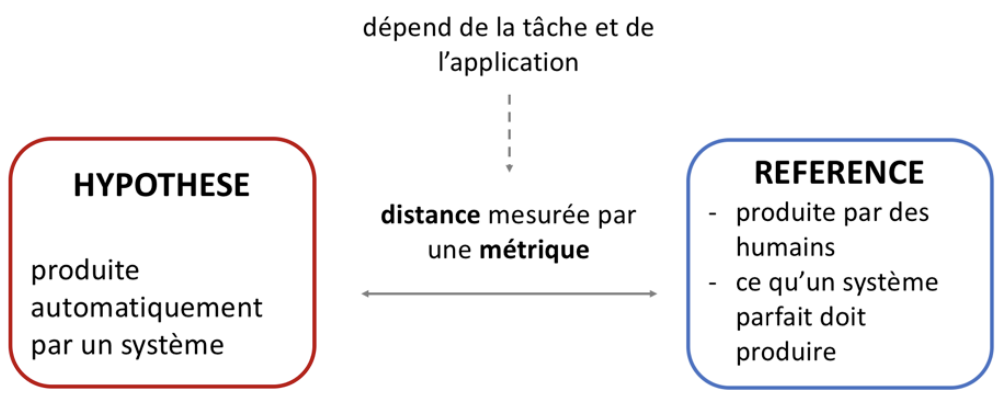
\includegraphics[width=.9\linewidth]{img/evaluation.png}
		\caption{Objectif : mesurer à quel point le système trouve les \og{}bonnes réponses\fg{}.}
		\label{fig:ling_out_TAL}
	\end{figure}
	
	Quelles \og{}bonnes réponses\fg{} ?
	\begin{itemize}
		\item traduction ou résumé automatique : bonnes réponses multiples
		\item \textsc{REN} : une seule et unique bonne réponse
	\end{itemize}
\end{frame}

\begin{frame}{Avantages et exigences}
	\begin{itemize}
		\item \textcolor{deepblue}{\textbf{Transparence}} : \og{}règles du jeu\fg{} connues par tous
		\item \textcolor{deepblue}{\textbf{Coût}} : réduit par rapport à une évaluation manuelle pour chaque hypothèse des systèmes
		\item \textcolor{deepblue}{\textbf{Reproductibilité}} : réutilisation au-delà des campagnes permettant une comparaison des résultats dans la production scientifique
	\end{itemize}
	
	Ce qu'il faut pour évaluer : 
	\begin{enumerate}
		\item une \bolder{métrique} mesurant la distance entre une référence et une hypothèse
		\item un \bolder{algorithme d'alignement} de la référence et de l'hypothèse
		\item un \bolder{algorithme de projection} des \textsc{EN} annotées sur la transcription manuelle de référence vers la transcription automatique
	\end{enumerate}
\end{frame}

\begin{frame}{Les mesures classiques}
	\bolder{Précision}
	
	Ratio entre le nombre de \textcolor{deepred}{réponses correctes} et toutes les \textcolor{deepred}{réponses données} par un système
	
	\begin{equation*}
		P = \dfrac{C}{C + S + I}
	\end{equation*}
	
	\begin{itemize}
		\item $C$ : nombre d'objets \textcolor{deepblue}{\textbf{corrects}} dans l'hypothèse
		\item $I$ : nombre d'\textcolor{deepblue}{\textbf{insertions}} par le système
		\item $S$ : nombre de \textcolor{deepblue}{\textbf{substitutions}} par le système (\textsc{EN} mal orthographiées)
		\item soit $C + S + I$ : nombre total d'objets dans l'hypothèse
	\end{itemize}
\end{frame}

\begin{frame}{Les mesures classiques}
	\bolder{Rappel}
	
	Ratio entre le nombre de \textcolor{deepred}{réponses correctes} et le nombre des \textcolor{deepred}{réponses attendues} (\textit{i.e.} présentes dans la référence)
	
		\begin{equation*}
		R = \dfrac{C}{C + S + D}
	\end{equation*}
	
	\begin{itemize}
		\item $D$ : nombre total d'\textcolor{deepblue}{\textbf{omissions}} (suppressions) opérées par le systèmes (\textsc{EN} non détectées, silence)
		\item $C + S + D$ : nombre total d'objets dans la référence
	\end{itemize}
\end{frame}

\begin{frame}{Exemple 1}
	\textcolor{deepred}{\texttt{REF}} : \texttt{<pers>Bertrand Delanoë</pers> a été élu maire de <loc>Paris</loc>}\\\medskip
	\textcolor{deepblue}{\texttt{HYP1}} :  \texttt{<pers>Bertrand Delanoë</pers> a été élu <pers>maire</pers> de <loc>Paris</loc>}
	
	\begin{itemize}
		\item Précision : $\dfrac{2}{3} = 0,67$
		\item Rappel :  $\dfrac{2}{2} = 1$
	\end{itemize}
	
	$\rightarrow$ ici \texttt{HYP1} produit du \bolder{bruit}.
\end{frame}

\begin{frame}{Exemple 2}
	\textcolor{deepred}{\texttt{REF}} : \texttt{<pers>Bertrand Delanoë</pers> a été élu maire de <loc>Paris</loc>}\\\medskip
	\textcolor{deepblue}{\texttt{HYP2}} :  \texttt{<pers>Bertrand Delanoë</pers> a été élu maire de Paris}
	
		\begin{itemize}
		\item Précision : $\dfrac{2}{2} = 1$
		\item Rappel :  $\dfrac{1}{2} = 0,5$
	\end{itemize}
	
	$\rightarrow$ \texttt{HYP2} produit du \bolder{silence}


	
\end{frame}

\begin{frame}{\textit{F}-mesure}
	Définie comme la moyenne harmonique entre Précision et Rappel :
	
	\begin{equation*}
		F = (1 + \beta^2) \times \dfrac{P \times R}{\beta^2 P + R}
	\end{equation*}
	
	où $\beta$ est un \textcolor{deepblue}{\textbf{poids}} permettant d'ajuster l'importance de $P$ ou $R$ (si 1, égale importance).
\end{frame}

\begin{frame}{Exemples}
		\textcolor{deepred}{\texttt{REF}} : \texttt{<pers>Bertrand Delanoë</pers> a été élu maire de <loc>Paris</loc>}\\\medskip
			\textcolor{deepblue}{\texttt{HYP1}} :  \texttt{<pers>Bertrand Delanoë</pers> a été élu <pers>maire</pers> de <loc>Paris</loc>}\\\medskip
	\textcolor{deepblue}{\texttt{HYP2}} :  \texttt{<pers>Bertrand Delanoë</pers> a été élu maire de Paris}
	
	\begin{equation*}
		F(HYP1) = (1 + 1^2) \times \dfrac{0,67 \times 1}{1^2 \times 0,67 + 1} = 0,80
	\end{equation*}
	
	\begin{equation*}
		F(HYP2) = (1 + 1^2) \times \dfrac{1 \times 0,5}{1^2 \times 1 + 0.5} = 0,67
	\end{equation*}
\end{frame}

\begin{frame}{Inconvénients des mesures classiques}
	\begin{itemize}
		\item fusionner $P$ et $R$ minimise le poids des erreurs d'insertion et d'omission par rapport aux erreurs de substitution, quel que soit $\beta$
		\item avec les typologies fines et complexes, besoin d'une métrique différenciant les erreurs
	\end{itemize}
	
			\textcolor{deepred}{\texttt{REF}} : \texttt{the <pers.ind>president of Ford</pers.ind>}\\\medskip
	\textcolor{deepblue}{\texttt{HYP1}} :  \texttt{the <pers.ind>president</pers.ind> of Ford} \\$\rightarrow$ erreur de frontière\\\medskip
	\textcolor{deepblue}{\texttt{HYP2}} :  \texttt{the <pers.coll>president of Ford</pers.coll>} \\$\rightarrow$ erreur de sous-type\\\medskip
		\textcolor{deepblue}{\texttt{HYP3}} :  \texttt{the <pers.coll>president</pers.coll> of Ford} \\$\rightarrow$ erreur de sous-type et de frontière
\end{frame}

\begin{frame}{Mesures basées sur le décompte d'erreurs : \textsc{SER}}
	\textsc{SER} : \textit{Slot Error Rate} \citep{makhoul1999performance}
	\begin{itemize}
		\item identique au \textit{WER} utilisé en reconnaissance autom. de parole
		\item utilisée lors de \textsc{ACE}, \textsc{ESTER-2}, \textsc{QUAERO} et \textsc{ETAPE}
		\item suppression du nombre d'insertion ($I$) du dénominateur
	\end{itemize}
	
	\begin{equation*}
		SER = \dfrac{S + D + I}{C + D + S} = \dfrac{S + D + I}{R}
	\end{equation*}
	
	où $R$ = nombre total d'\textsc{EN} de la référence
\end{frame}

\begin{frame}{\textsc{SER}}
	Possibilité d'affiner l'importance relative des erreurs
	
	\begin{equation*}
		SER = \dfrac{\alpha_1S_t + \alpha_2S_f + \beta D + \gamma I}{R}
	\end{equation*}
	
	\begin{itemize}
		\item $S_t$ et $S_f$ : nb total de substitutions de type et de frontières
		\item $D$ et $I$ : nombre total d'omissions et d'insertions
		\item $\alpha_1$, $\alpha_2$, $\beta$ et $\gamma$ : poids affectées à chaque catégories d'erreur
	\end{itemize}
\end{frame}
%\begin{frame}{Appliquer les annotations dans le texte}
%\textcolor{deepblue}{Annoter le texte}
%		\begin{itemize}
%		\item ouvrir un texte (p. ex. le \textit{Tour du monde en 80 jours})
%		\item puis, menu \Colorbox{mygray}{\lstinline|Text > Locate Pattern > Graph|}
%		\item selectionner \Colorbox{mygray}{\lstinline|Grammar Outputs > Merge with input text|}
%	\end{itemize}
%			\begin{figure}[h] % Use [H] to force the figure to stay in place
%		\centering
%		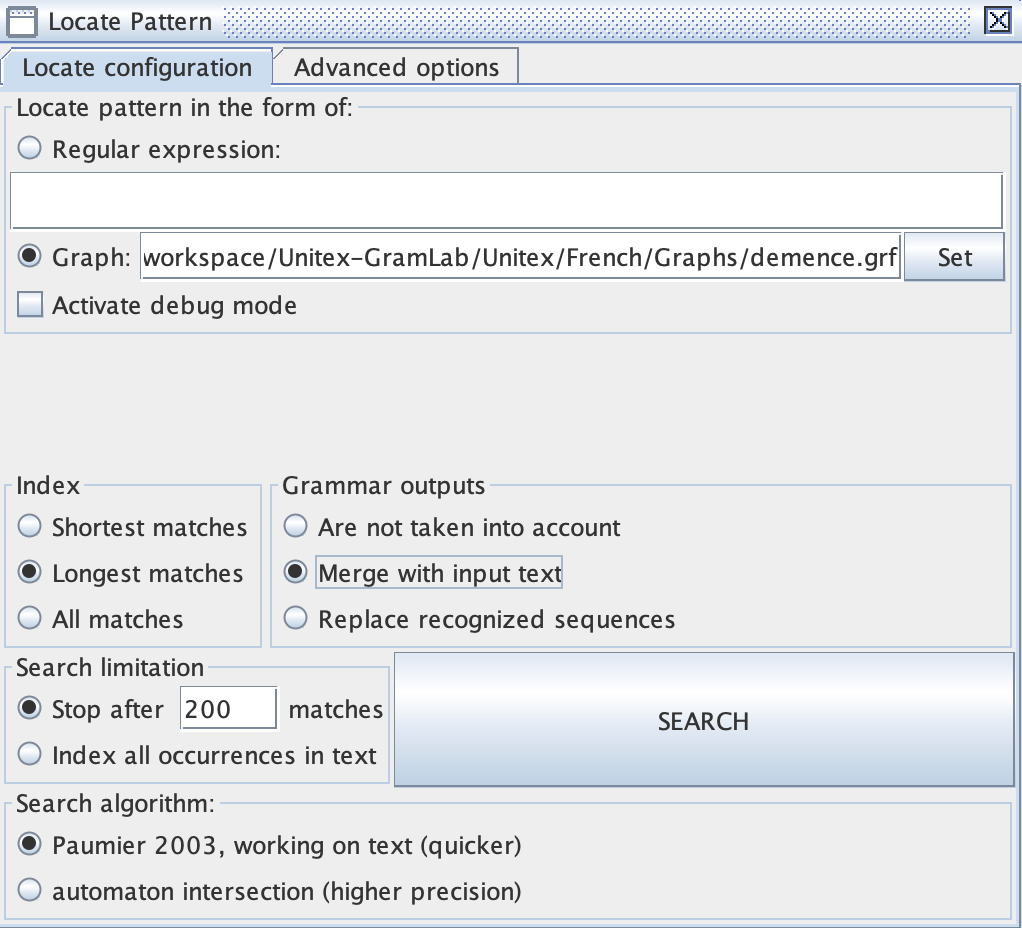
\includegraphics[width=.4\linewidth]{img/merge.png}
%		\caption{Appliquer les annotations.}
%		\label{fig:ling_out_TAL}
%	\end{figure}
%\end{frame}

\begin{frame}[allowframebreaks]
		\printbibliography
\end{frame}




\begin{frame}{Licence}
	\centering
	{\small Le contenu de cette présentation est sous licence \texttt{CC-BY-NC-SA 4.0}\\Utilisation non commerciale -- Partage dans les mêmes conditions.\\}
	\href{https://creativecommons.org/licenses/by-nc-sa/4.0/deed.fr}{\ccbyncsa}
\end{frame}

\end{document}